{\it Section prepared by the Working Group: 'Prospects for boosted top quarks',  A. Altheimer, J. Ferrando, \underline{J. Pilot}, S. Rappoccio, M. Villaplana, \underline{M. Vos}.
}

Among the many applications of the strategies for boosted objects
discussed in the literature 
(the bibliography of References~\cite{Abdesselam:2010pt,Altheimer:2012mn} is
a good starting point to navigate the extensive literature), the study of 
highly energetic top quarks forms 
the case that has been studied in greatest detail by the experiments. 
Several studies of the production of boosted top
quarks have set limits on new physics scenarios. The first sample 
of boosted top quarks has also been used to understand the 
modelling of the parton shower and the detector response. In this section
we present a summary of achievements so far, discuss how existing
analyses could benefit from an improved understanding of jet substructure,
and explore possible directions for future work.

\subsection{Boosted top quark production}

\begin{table*}[htbp!]
\centering
%\setlength\fboxsep{0pt}
%\setlength\fboxrule{0.25pt}
\caption{The top pair production rate at past, present and future colliders, 
calculated with the MCFM code~\cite{Campbell:2010ff}. The inclusive 
production rate 
is given in the first row. The expected number of events with boosted 
top quarks ($M_{t\bar{t}} > $ 1~\tev) and highly boosted top quarks 
($M_{t \bar{t}} > $ 2~\tev) is given in the second and third row, respectively.}
\begin{tabular}{|l|c|c|c|c|} \hline
Collider \& phase & Tevatron run II & LHC 2012 & LHC phase II & HE-LHC \\
process \& energy,  &  $ p \bar{p}$ at $\sqrt{s} = $ 1.96~\tev & $pp $ at  $\sqrt{s} = $8~\tev &  $pp $ at  $\sqrt{s} = $13~\tev & $pp $ at  $\sqrt{s} = $33~\tev \\
integrated luminosity      & $\mathcal{L} =$ 10~\ifb{}  & $\mathcal{L} =$ 20~\ifb{} & $\mathcal{L} =$ 300~\ifb{} & $\mathcal{L} =$ 300~\ifb{}  \\ \hline
Inclusive $t \bar{t}$ production & 6 $\times $ 10$^{4}$ & 4 $\times$ 10$^6$ & 2 $\times $ 10$^8$ & 1.4 $\times $ 10$^9$  \\ \hline
Boosted production & 23 &  6 $\times $ 10$^{4}$ &  5.2 $\times$ 10$^6$ &  7.1 $\times$ 10$^7$ \\ \hline
Highly boosted & 0 &  500 &  1.1 $\times$ 10$^5$ & 3.9 $\times$ 10$^6$ \\ \hline
\end{tabular}
\label{tab:boostedtoprates}
\end{table*}


The top quark decay topology observed in the detector depends strongly on the
kinematic regime.  The decays products of top quarks produced nearly at rest 
($p_T < 200$ GeV/$c$) are well-separated, leading to experimental signatures
such as isolated leptons and a relatively large number of clearly resolved 
jets. With increasing transverse momentum, the decay products 
of the top quark will become collimated and possibly reconstructed in the 
same final state object. For intermediate boosts (200 $< p_T < $400~\gev{}), 
the daughters of the $W$ boson from a fully-hadronic top decay will be close 
enough to be clustered into the same jet.  At this point, the use of jet 
substructure techniques becomes important to efficiently identify these decay 
signatures. At even larger $p_T$ top quarks become truly boosted objects: 
all decay products of the top will be 
strongly collinear, with the $\Delta R \sim 2 m_{\mathrm{top}} / p_T$.  
Hadronic top quarks can be reconstructed in a single 
jet, and top quarks with leptonic decays generally contain non-isolated 
leptons due to the overlap with the $b$-quark jet.  




Table~\ref{tab:boostedtoprates} presents the expected numbers of 
boosted top quark pairs according to the Standard Model at past, present and 
future colliders. The numbers show clearly how the study of boosted top quarks 
becomes viable only with the start of the LHC. The first phase of operation
yields a sample of several tens of thousands of boosted top quark pairs.
The next-to-last column indicates the size of the 
sample expected in a 13 or 14~\tev{} run of the LHC, that is to start 
by the end of 2014. The increase in the centre-of-mass 
energy and the larger integrated luminosity each bring an increase 
of an order of magnitude in the production of boosted top quarks. 


We expect, therefore, that boosted topologies will gain considerable importance 
as the LHC program develops. To exploit the LHC data to their full potential it 
is  critical that existing experimental strategies are adapted to this
challenging kinematical regime. Before we turn to the results of 
analyses of boosted object production, we discuss a number of new tools
that were developed to identify and reconstruct boosted top quarks efficiently. 


\subsection{Top Tagging.}  

Excellent reviews of top tagging algorithms exist~\cite{Plehn:2011tg}. 
Previous BOOST reports have compared their 
performance for simulated events (at the particle level). In this 
Section we present a very brief review for completeness. 

The Johns Hopkins (JHU) tagger \cite{Kaplan:2008ie} identifies 
substructure by reversing through the iterative clustering process 
used to form jets.  Subjets are found using several criteria -- the 
ratio of their individual $p_T$ to the original jet $p_T$ must be above 
a given threshold, and the subjets must be spatially separated from each 
other to give a valid decomposition.  In this way, a jet can be 
deconstructed into up to four subjets, and jets with three or more 
subjets are analyzed further, requiring the invariant mass of the 
identified subjets to be in the range $[145, 205]$~\gev{}, and two 
of the subjets to be consistent with $m_W$, in the range $[65,95]$~\gev.  
There is an additional cut on the $W$ boson helicity angle, 
$\cos \theta_h < 0.7$. 

The variant of the JHU tagger used by CMS\cite{CMS-PAS-JME-09-001} uses 
a similar jet decomposition, with slight differences in the selections of 
top quark and $W$ boson masses from the subjets.  Additionally, the CMS 
top tagger does not apply the $W$ boson helicity angle requirement, but
instead selects jets with the
minimum pairwise mass of the subjets larger than 50~\gev.
The JHU and CMS top tagging algorithms have been developed with jet 
distance parameters up to $R = 0.8$, and therefore are only efficient 
for top quarks with $p_T$ above approximately 400 GeV/$c$.  

The HEP top tagger \cite{Plehn:2010st}, is designed to use jets with 
distance parameter $R=1.5$, thereby extending the reach of the tagging 
algorithm to lower jet $p_T$ values.  The algorithm uses a mass drop 
criterion to identify substructure within the jet, but also uses a 
filtering algorithm to remove soft and large-angle constituents from the 
individual subjets.  The three subjets with a combined mass closest to 
$m_t$ are then chosen for further consideration.  Cuts are then applied 
to masses of subjet combinations to ensure consistency with $m_W$ and 
$m_t$.  Specifically, for the three subjets sorted in order of subjet 
$p_T$, having masses $m_1, m_2, m_3$, the quantities $m_{23}/m_{123}$ 
and $\arctan m_{13}/m_{12}$ are computed.  Geometrical cuts can be 
applied in the phase space defined by these two quantities 
to select top jets and reject quark or gluon jets.  

The HEP top tagger obtains tagging efficiencies of up to 37\% for lower 
$p_T$ top quarks ($p_T > 200$ GeV/$c$), with an acceptable mistag rate.  
It has been used by the ATLAS \ttbar{} resonance search in the fully
hadronic channel~\cite{Aad:2012raa}, where no {\it resolved} analysis
has been performed. At high jet $p_T$, the efficiencies for the HEP Top 
Tagger and JHU Top Tagger selections are comparable.

Boosted top quarks were also studied using both $R=1.0$ anti-$k_{t}$ jets 
and jets identified by the HEPTopTagger~\cite{Plehn:2010st} algorithm 
as candidate ``top-jets.'' Kinematic and substructure distributions were 
compared between data and MC simulation and were found to be in agreement. 
Furthermore, the efficiency with which top quarks were identified as such 
was found to be significantly increased in both cases, and the HEPTopTagger 
was shown to reduce the backgrounds to such searches dramatically, even 
with a relatively relaxed transverse momentum selection.

Overall, the results from ATLAS suggests that, among the jet grooming 
configurations tested, the trimming algorithm exhibited an improved mass 
resolution and smaller dependence of jet kinematics and substructure 
observables on pile-up (such as 
$N$-subjettiness~\cite{Thaler:2010tr,Thaler:2011gf} and the 
$k_{t}$ splitting scales~\cite{Butterworth:2002tt}) compared to the 
pruning configurations examined. For boosted top quark studies, 
the anti-$k_{t}$ algorithm with a radius parameter of $R=1.0$ and 
trimming parameters $f_{\rm cut}=0.05$ and $R_{\rm sub}=0.3$ was found to 
be optimal, where a minimum $p_{T}$ requirement of 350 GeV is typical. It 
is important to note that only the $k_{t}$-pruning for $R=1.0$ jets was 
tested and that since the performance does depend somewhat on this 
parameter, further studies are necessary to optimize for other jet size. 
Lastly, Cambridge-Aachen jets with $R=1.2$ using the mass-drop filtering 
parameter $\mu_{\rm frac}=0.67$ were found to perform well for 
boosted two-pronged analyses such as $H\rightarrow b\overline{b}$ or 
searches involving boosted $W\rightarrow q\overline{q}$ decays.

A final algorithm that is currently being investigated is the $N$-subjettiness 
algorithm \cite{Thaler:2010tr} presented in Section~\ref{sec:mc}. 


Several new techniques and ideas are emerging, that aim to improve 
boosted top identification and reconstruction.

One such technique is that of shower deconstruction \cite{Soper:2010xk}.  
This method aims to identify boosted hadronic top quarks by computing the 
probability for a top quark decay to produce the observed jet, including its 
distribution of constituents.  The probability for the same jet to have 
originated from a background process is also computed.  These probabilities 
are computed by summing over all possible shower formations resulting in the 
observed final state, accounting for different gluon splittings and 
radiations, among other processes. This is done both for the signal shower 
processes and background shower processes. A likelihood ratio is formed 
from the signal and background probabilities and used to discriminate 
boosted top quarks from generic QCD jets.  The process of evaluating all 
shower histories can be computationally intensive, so certain requirements 
are made on the number of constituents used in the method to make the 
problem tractable.  The results presented in Ref.~\cite{Soper:2012pb} 
show an improvement on the top taggers described previously. Specifically, 
the shower deconstruction method reduces the top mistag rate by a factor 
of 3.6 compared to the JHU top tagger, while maintaining the same signal 
acceptance.  This method is also applicable to the lower $p_T$ regime, 
and there improves upon the top mistag rate from the HEP top tagger by a 
factor of 2.6, again keeping identical signal efficiency.

\begin{figure*}[htpb!]
\begin{center}
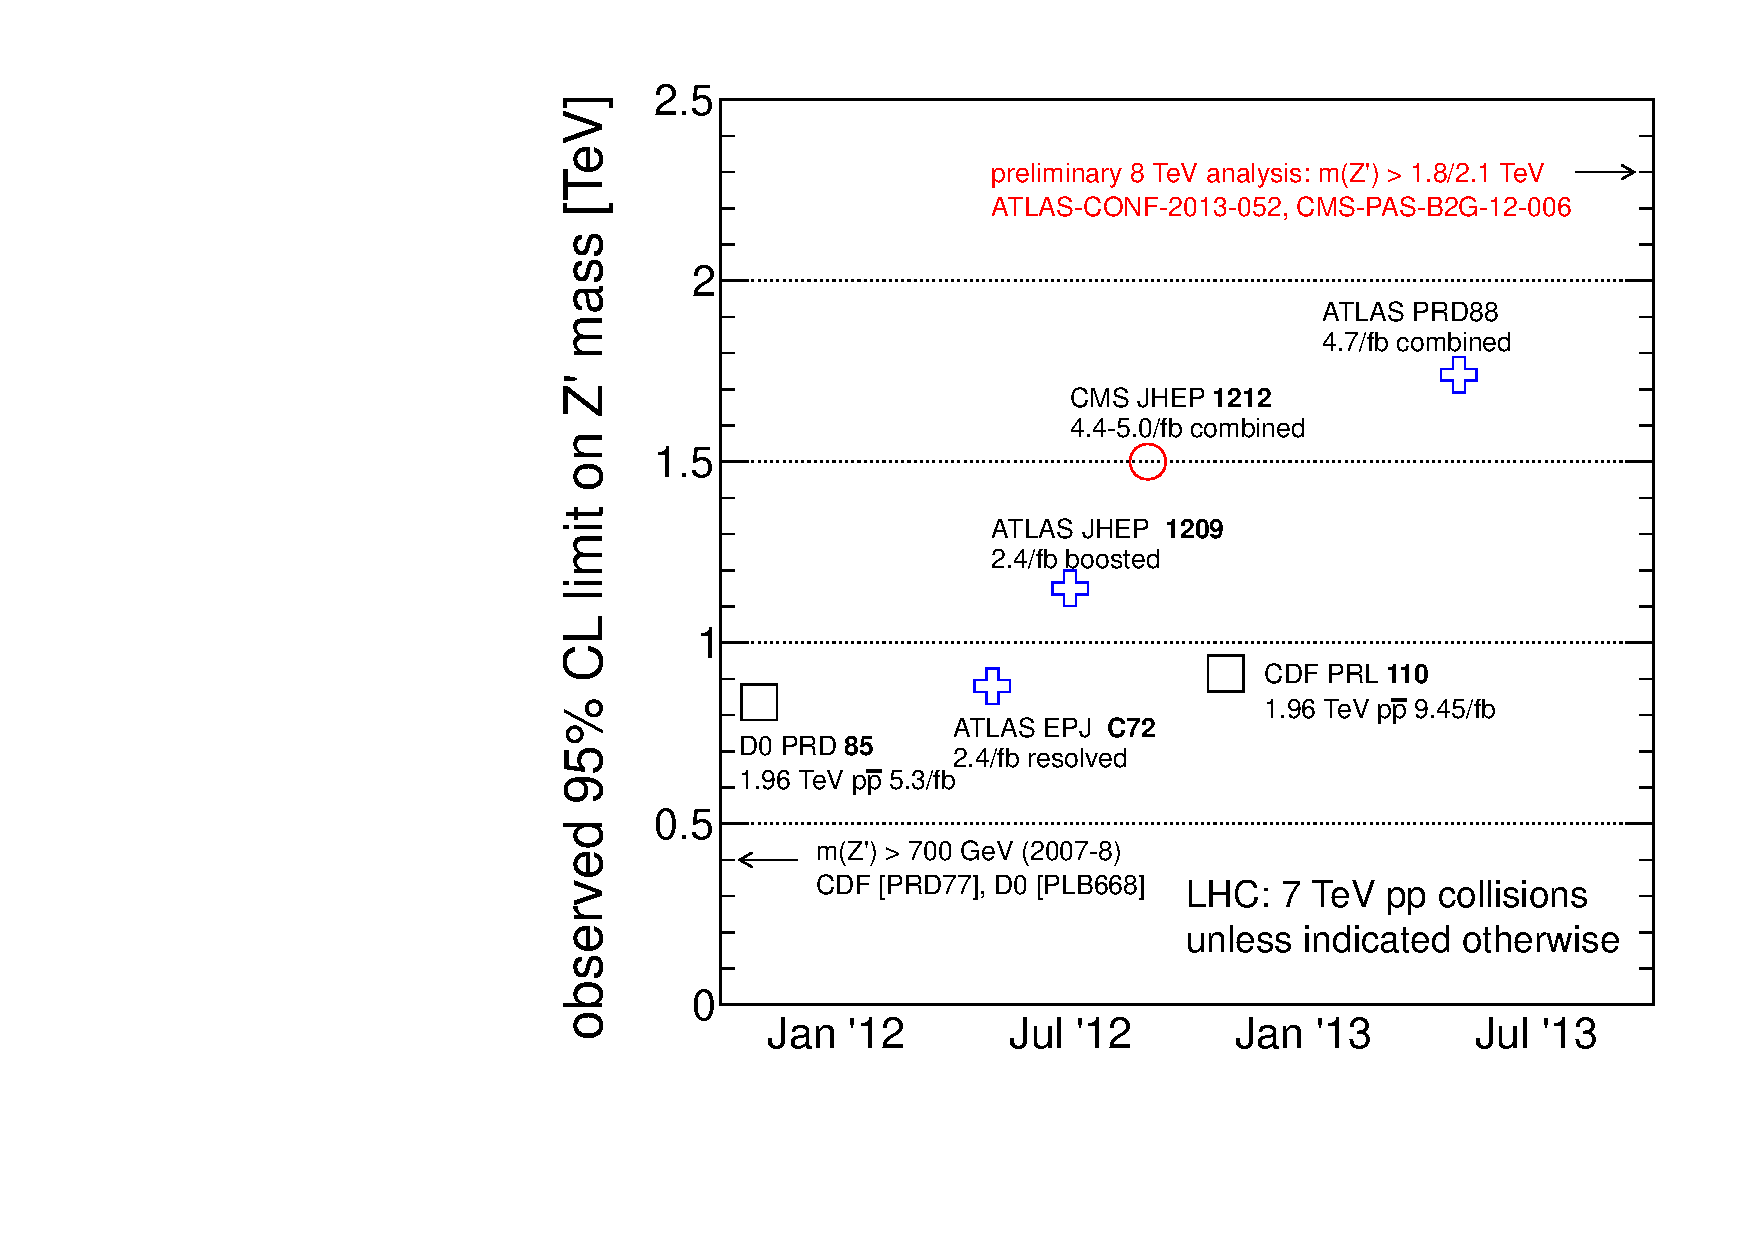
\includegraphics[width=0.6\linewidth]{summary_resonance_searches}
\end{center}
\caption{Overview of evolution of the sensitivity of $t\bar{t}$ resonance searches in the first years of LHC operation. The sensitivity is presented in terms of the lower limit on the mass of a narrow $\Zprime$ boson. The production rate for this new state is given by a benchmark model that is common to all experiments (a leptophobic topcolor $\Zprime{}$ boson).}
\label{fig:summary_searches}
\end{figure*}

\begin{table*}[htpb!]
\begin{center}
\caption{Exclusion limits at 95\% confidence level for a narrow $\Zprime{}$ boson, as obtained in \ttbar{} resonance searches at the Tevatron and the first years of operation of the LHC.}
\vspace{2mm}
\begin{tabular}{lccccc}
\hline 
CDF and D0 References                        &  ~\cite{Aaltonen:2007ag} & ~\cite{Abazov:2008ny} &  ~\cite{Aaltonen:2011vi} & ~\cite{Abazov:2011gv} & ~\cite{Aaltonen:2012af}\\
Final state   \&                 & $l$+jets & $l$+jets & fully had. & $l$+jets & $l$+jets \\   
Reconstruction                   &  resolved & resolved & resolved & resolved & resolved \\  
$\sqrt{s}$ [\tev{}] & 1.96 &  1.96 &  1.96 & 1.96  & 1.96  \\
$\int{L} $ [~\ifb{}] & 1~\ifb{} & 1~\ifb{} &  4~\ifb{}  &  4~\ifb{} & 10~\ifb{} \\
\Zprime{} mass [TeV]  & $<$ 0.7 & $<$ 0.720 & $<$ 0.805 &   $ < $  0.835 & $ < $ 0.915  \\ \hline
ATLAS Reference                        &     ~\cite{Aad:2012wm}     &  ~\cite{Aad:2012dpa}  &  ~\cite{Aad:2012raa}  & ~\cite{Aad:2013nca}  &  ~\cite{ATLAS-CONF-2013-052} \\
Final state   \&                 & $l$+jets & $l$+jets & fully had. & $l$+jets & $l$+jets \\   
Reconstruction                   & resolved & boosted & boosted & combined & combined \\ 
$\sqrt{s}$ [\tev{}] &  7&  7 & 7  & 7 & 8 \\
$\int{L} $ [~\ifb{}] & 2.04~\ifb{} &   2.04~\ifb{} &  4.07~\ifb{}  &  4.07~\ifb{} & 14~\ifb{} \\
\Zprime{} mass [TeV]  & 0.5 $-$ 0.88 & 0.6 $-$ 1.15 & 0.7$-$1, 1.28$-$1.32  &   $ < $  1.74 & $ < $ 1.8 \\
$g_{KK} $ mass [TeV]  & 0.5 $-$ 1.13 & 0.6 $-$ 1.5  & 0.7 $-$ 1.62 & $<$ 2.07 & $ < $  2.0 \\ \hline 
CMS Reference                        &  ~\cite{Chatrchyan:2012ku}  &  ~\cite{Chatrchyan:2012cx}  & ~\cite{Chatrchyan:2012yca}  &  ~\cite{CMS-PAS-B2G-12-005} & ~\cite{CMS-PAS-B2G-12-006}\\
Final state   \&                 & fully hadronic  & $l$+jets & di-lepton & fully hadronic & $l$+jets\\   
Reconstruction                   & boosted         & combined &          & boosted & combined  \\ 
$\sqrt{s}$ [\tev{}] & 7 &  7 & 7  & 8 & 8 \\
$\int{L} $ [~\ifb{}] & 5.0~\ifb{} & 4.4$-$5.0~\ifb{} &   5.0~\ifb{} &  19.6~\ifb{}  &  19.6~\ifb{}  \\
\Zprime{} mass [TeV]  & 1.3 $-$ 1.5 & $ < $1.49 & $ < $1.3  & $ < $ 1.7 &   $ < $  2.1   \\
$g_{KK} $ mass [TeV]  &  1.4 $-$ 1.5  & $ < $1.82 & $ < $1.8  & $ < $ 1.8 & $ < $ 2.5   \\ \hline 
\end{tabular}
\label{tab:limits}
\end{center}
\end{table*} 

Another algorithm under development is the template 
overlap method~\cite{Backovic:2012jj}. The template overlap method 
is designed for use in boosted top identification as well as boosted Higgs 
identification.  The method is similar to that of shower deconstruction, 
in that it attempts to quantify how well a given jet matches a certain 
expectation such as a boosted top quark or boosted Higgs decay. However, 
this method uses only final state configurations, whereas the shower 
deconstruction method takes into account the showering histories. A catalog 
of templates is formed by analyzing signal events. Once this is in place, 
individual jets can be analyzed by evaluating an overlap function which 
evaluates how well the current jet matches the templates from the signal 
process of interest.  For example, a template for hadronic boosted top 
quark decays would consist of three energy deposits within the jet. In 
studies with high-$p_T$ jets, the rejection factor of QCD jets compared 
to jets from boosted top quark decays is of the order 10$^2$. One additional 
feature of this template overlap method is the automatic inclusion of 
additional parton radiation into the template catalog, such as for Higgs 
decays to bottom quark pairs, where there is commonly an additional gluon 
radiated, resulting in 3 energy deposits instead of the 2 from the $b$ quarks.

Finally, the Q-jets~\cite{Ellis:2012sn} scheme could be used for top-tagging.
This is a method to remove dependence of analysis results on the choice of 
clustering algorithm used to reconstruct jets.  For example, one could use 
either the Cambridge-Aachen algorithm or the kT algorithm to cluster jets, 
and may obtain significantly different results in the jet masses.  The 
Q-jets algorithm attempts to use all possible ``trees'' to cluster 
constituents, rather than using the single tree provided by the specific 
clustering algorithm used.  In this way, each jet now has a distribution 
of possible masses instead of a single jet. This provides additional 
information which can enhance signal discrimination. For example, the 
variance of the jet mass between individual clustering trees can be examined, 
rather than relying on just a single value. The statistical stability is 
also enhanced when using the Q-jets algorithm.

\subsection{Searches with boosted top quarks}





The first area where new tools developed specifically for the selection and 
reconstruction of boosted top quarks have shown their value is in searches for 
massive new states decaying to top quark pairs. The first application 
of techniques specifically aimed at boosted top decays was the CMS 
\ttbar{} resonance search in the all-hadronic channel~\cite{Chatrchyan:2012ku}.
The evolution of the 
mass reach~\footnote{The sensitivity to massive particles is expressed in terms
of the observed 95 CL lower limit on the mass of a leptophobic topcolor \Zprime{} 
boson. The motivation of this particular model may not have survived recent 
advances in particle physics, but to monitor the sensitivity
of searches it is still the best benchmark on the market.} 
of \ttbar{} resonance searches in the more sensitive 
``lepton+jets'' channel is shown in 
Fig.~\ref{fig:summary_searches}. 
By the start of the LHC program the Tevatron experiments had excluded a \Zprime{} boson
mass lower than 700~\gev{}~\cite{Aaltonen:2007ag,Abazov:2008ny}. In the course of 2011 and 2012 
the limit was extended to 800~\gev{} by a D0 search on nearly 5~\ifb{}~\cite{Abazov:2011gv} 
and to approximately 900~\gev{} by a CDF analysis of
the complete Tevatron data set~\cite{Aaltonen:2012af}.
An ATLAS search on 2.4~\ifb{} of 7~\tev{} LHC data~\cite{Aad:2012wm} collected 
in 2011 reached a
similar precision. All these analyses followed the conventional, {\it resolved}
approach that is based on the assumption that the six fermions from the decay of
the top quark pair
($t \rightarrow W^+ b \rightarrow l^+ \nu_l b$ and the charge conjugate process)
can be resolved individually.


In some cases ATLAS and CMS analyses specifically designed for boosted top quarks~\cite{Aad:2012dpa,Chatrchyan:2012cx} scrutinized the same data set that had been used by the {\it resolved} approach.
A direct comparison of these results demonstrates that the novel approach has considerably better sensitivity for massive 
states~\cite{Aad:2012dpa}. The final analyses on 2011 data~\cite{Aad:2013nca,Chatrchyan:2012cx} combine {\it resolved}
and {\it boosted} methods to attain good 
sensitivity over the complete mass spectrum. The excluded mass range is pushed 
up to 1.74~\tev{}.

Searches in the ``lepton+jets'' channel are complemented by analyses of the fully hadronic
($t\bar{t} \rightarrow 6$ jets) and di-lepton ($t\bar{t} \rightarrow b \bar{b} l^+ \nu_l l'^- \bar{\nu}_l'$) decay chains. 
Only one fully hadronic \ttbar{} resonance search was performed at the Tevatron~\cite{Aaltonen:2011vi}.
At the LHC, with a daunting multi-jet background, these searches are even more challenging. 
The advent of new algorithms has, however, greatly boosted their potential. The mass reach of the
CMS~\cite{Chatrchyan:2012ku} and ATLAS search~\cite{Aad:2012raa} are compared to that of the
``lepton+jets'' searches in Table~\ref{tab:limits}. 

The prospects for progress are good. Preliminary results on the 2012 data 
set~\cite{ATLAS-CONF-2013-052,CMS-PAS-B2G-12-005,CMS-PAS-B2G-12-006} 
have significantly extended previous limits.

\subsection{Jet substructure performance and searches}

The results in the previous Section demonstrate the proof-of-principle: 
the addition of jet substructure to the experimentalists' tool-box 
boosts the sensitivity of searches for new physics at the LHC. 
It is clear, however, that these tools are
still in their infancy. In all searches discussed in the previous Section 
large systematic uncertainties are assigned to the large-R jets. 
It is natural to suspect that further progress could be made with better 
(and, especially, better understood) tools. 

To quantify the impact of the jet-related systematics on the sensitivity we
have evaluated expected limits on the narrow \Zprime{} boson with all sources
of systematic uncertainty, except one (so-called $N-1$ limits) in several
iterations of the ATLAS searches in the lepton+jets final state. The
uncertainties associated with the large-R jet that captures the 
hadronic top decay are always the dominant source of uncertainty. 
Their impact is considerably larger than that of systematics 
associated with the narrow jets, even at relatively low resonance mass.
The limits
over a large mass range (1-2~\tev{}) would improve by approximately 5-10\% if 
only the uncertainty on the scale and resolution of mass and energy of
anti-$k_t$ jets with $R=1$ is removed. 

If we apply an ad hoc scale factor
of two to this uncertainty (representing a failure to bring these
uncertainties under control) we find that the sensitivity is further degraded. 
A significant reduction of large-R 
jet uncertainties, on the other hand,
brings the $N-1$ limits with no jet-related systematics and the 
limits with reduced large-R jet systematics to within
2\%. 

CMS has not published the $N-1$ results for their searches, but 
qualitatively the same picture emerges. In the fully
hadronic searches the jet-related uncertainties have the largest
impact on the limits.

We conclude that further progress undertanding jet substructure 
still has substantial
potential to increase our sensitivity to massive new states decaying 
to top quarks.

\subsection{Further applications}

The selection for boosted top quarks, in the lepton+jets and fully hadronic
channels, have proven their value in \ttbar{} resonance searches, but
are more generally applicable. 

The obvious direction to extend the 
range of applications is to other searches with boosted top quarks.
The $W' \rightarrow tb$ that are currently performed in the channel
where the top quark decays to a charged lepton, neutrino and b-jet.
We expect, however, that, ultimately the highest mass reach should
be obtained in the hadronic decay (with a factor two large branching
ratio if $\tau$-leptons are not considered).

We expect differential cross-section measurements for \ttbar{} to benefit
from these techniques at large transverse momentum and invariant mass
of the \ttbar{} pair. Apart from the better selection efficiency in
algorithms designed for this kinematic regime, the 
better truth-to-reconstructed mapping of $p_T$ and $m_{\ttbar}$ 
is expected to be an important advantage. We are looking forward to 
such measurements from the ATLAS and CMS experiments.
Also analyses that rely
strongly on the reconstruction of the top quark direction, such as
the charge asymmetry measurement, should benefit.

Finally, several authors~\cite{Plehn:2009rk} have commented on the potential
of events with mildly boosted top quarks for the observation of $t\bar{t}H$
and a measurement of the  production rate.


\subsection{Summary}

Over the last five years, many ideas have been proposed to cope with the 
challenge of boosted top quark reconstruction. Since then, these ideas
have been implemented by the experiments and put to the test, primarily
in searches for massive new states decaying to \ttbar{} pairs. The overview
we presented in Fig.~\ref{fig:summary_searches} and Table~\ref{tab:limits}
is a testimony to the increase of sensitivity for such states fuelled
by the performance of the LHC.
Such progress would not have been possible if novel techniques for the 
study of boosted top quarks had not been developed.
We expect the selection developed for the lepton+jets and fully hadronic
to find further applications in searches and measurements.
